%
% Шаблон магистерской диссертации
%

\documentclass[a4paper,12pt]{article}
\usepackage[backend=biber,sorting=none,style=gost-numeric,autolang=other]{biblatex} % библиография
\usepackage{mathtext} %русские буквы в формулах
\usepackage[T2A]{fontenc}
\usepackage[utf8]{inputenc}
\usepackage[english,russian]{babel}
\usepackage{amsmath}
\usepackage{fancyvrb}
\usepackage{formular}
\usepackage{setspace} % управление междустрочными интервалами
%поля документа
\usepackage[left=3cm,right=1.5cm,top=2.5cm,bottom=2.5cm]{geometry}

\usepackage{misccorr} % точки в конце номеров разделов, использовать перед пакетом ccaption!
\usepackage{ccaption} % изменения подписей к рисункам и табл.

\usepackage[nooneline]{caption} 
\captionsetup[table]{justification=raggedright} % заголовок таблицы выравнивается влево
\captionsetup[figure]{justification=centering,labelsep=endash} % заголовок рисунка - по центру

% отступ перед первым абзацем
\usepackage{indentfirst}
%вставка изображений
\usepackage{graphicx}
% счетчики
\usepackage{totcount}
% управление содержанием
\usepackage{tocloft}
% управление таблицами и рисунками
\usepackage{float}

\newcounter{mycitecount}                                %% Счётчик библиографии
\AtEveryBibitem{\stepcounter{mycitecount}}              %% Работает для biblatex

\usepackage[figure,      %
            table,       %
            mycitecount, xspace ]{totalcount}           %% Подсчёт общего количества объектов в документе

% окружение для листингов - с нумерацией строк слева
\DefineVerbatimEnvironment{MyCode}{Verbatim}{frame=lines,numbers=left,numberblanklines=false,framesep=5mm}

% автоматическая нумерация листингов
\newfloat{Program}{phb}{lop}
\floatname{Program}{Листинг}
\floatstyle{ruled}

\setcounter{secnumdepth}{3} % глубина нумерации до подразделов

%если нужны точки в оглавлении для разделов - раскомментируйте следующую команду
%\renewcommand{\cftsecleader}{\cftdotfill{\cftdotsep}}

\addto\captionsrussian{%
\renewcommand{\figurename}{Рисунок}%
\renewcommand{\tablename}{Таблица}%
}

% дефис в подписи к рисункам
\captiondelim{ -- } 

% Настройки для окружений с подчеркиваниями для подписей и пр.
\setFRMfontencoding{T2A}
\setFRMdfontencoding{T2A}
% thanks to A.Starikov
\setFRMfontfamily{cmr}
\setFRMdfontfamily{ptm}
\setFRMdfontsize{10pt}

% задает длину поля для подписи на титульной странице
\newFRMfield{xtitlesign}{32mm}

% поле для факультета или кафедры
\newFRMfield{fcath}{65mm}

%имя файла с библиографией в формате BibTex
\addbibresource{rbiblio.bib}

\begin{document}

% счетчики страниц, рисунков, таблиц
\regtotcounter{page}
\regtotcounter{figure}
\regtotcounter{table}

\renewcommand{\refname}{\centerline{СПИСОК ИСПОЛЬЗОВАННОЙ ЛИТЕРАТУРЫ}} 
\renewcommand{\contentsname}{\centerline{СОДЕРЖАНИЕ}} 
%\renewcommand{\refname}{Список источников}  % По умолчанию "Список литературы" (article)
%\renewcommand{\bibname}{Литература}  % По умолчанию "Литература" (book и report)

% титульная страница
\thispagestyle{empty}
\begin{center} \small
\textbf{МИНИСТЕРСТВО ОБРАЗОВАНИЯ И НАУКИ РОССИЙСКОЙ ФЕДЕРАЦИИ}\\
ФЕДЕРАЛЬНОЕ ГОСУДАРСТВЕННОЕ АВТОНОМНОЕ ОБРАЗОВАТЕЛЬНОЕ УЧРЕЖДЕНИЕ
ВЫСШЕГО  ОБРАЗОВАНИЯ\\
«Национальный исследовательский ядерный университет «МИФИ»\\
\textbf{Обнинский институт атомной энергетики} – \\
филиал федерального государственного автономного образовательного учреждения высшего\\
образования «Национальный исследовательский ядерный университет «МИФИ»\\
(ИАТЭ НИЯУ МИФИ)
\end{center}
%\vfill
\medskip

% Направление подготовки следует уточнять,
% магистры и бакалавры могут иметь разные наименования
\begin{center}
\begin{tabular}{rl}
Отделение & \useFRMfield{fcath}[\large Интеллектуальные кибернетические системы] \\ 
%Направление подготовки & \useFRMfield{fcath}[\large Информационные системы и технологии] \\ 
\end{tabular} 
\end{center}

\vfill

\large 

\begin{center}
\textbf{\Large Выпускная квалификационная работа --- } \\
\textbf{\Large магистерская диссертация}\\
	
	\medskip
по направлению подготовки: \textbf{09.04.02 Информационные  \\ системы и технологии}\\

Направленность (профиль): \textbf{Информационные системы}
	
\vfill
\vfill
\medskip

\textbf{\Large 
	<<Контроль электроэнергии и водоснабжения в рамках Умного города>>
}

\end{center}

\vspace{1cm}

\begin{tabular*}{\textwidth}{p{78mm}p{33mm}p{64mm}}
Выполнил:\\студент гр. ИС-М18 & \useFRMfield{xtitlesign} & Кузнецов~А.В.\\
& & \\
Руководитель ВКР,\\
профессор отделения ИКС, \\
докт.техн.наук & \useFRMfield{xtitlesign} & Яцало~Б.И. \\
& & \\

Нормоконтроль & \useFRMfield{xtitlesign} & Пичугина~И.А. \\
& & \\
% Если нужно добавить консультанта - раскомментируйте две строчки ниже
%Консультант ВКР бакалавра\\организация, должность, звание  & \useFRMfield{xtitlesign} & К.О.Нсультант\\
%& & \\
%	Рецензент\\к.ф.-м.н.,   & \useFRMfield{xtitlesign} & В.А. Чепурко\\

& & \\
Выпускная квалификационная \\ работа допущена к защите & \useFRMfield{xtitlesign} &  \\
& & \\
Руководитель\\ образовательной программы \\
09.04.02 Информационные системы и технологии,\\
докт.техн.наук  & \useFRMfield{xtitlesign} &Яцало~Б.И. \\

\end{tabular*}


\vfill
\large

\begin{center}
Обнинск, 2020 г
\end{center}

\onehalfspacing

\pagebreak

% реферат
\thispagestyle{empty}

\section*{\centering РЕФЕРАТ}

\total{page} стр., \total{table} табл., \total{figure} рис., \totalmycitecounts ист. 

УМНЫЙ ГОРОД, ИНТЕРНЕТ ВЕЩЕЙ, СИСТЕМА УЧЕТА РЕСУРСОВ, ПРИБОР УЧЕТА, АНАЛИЗ ДАННЫХ, POSTGRESQL, JAVA

Данная магистерская диссертация посвящена разработке программного обеспечения системы учета ресурсов в жилых зданиях с использованием аппаратной части для сбора данных с контроллеров приборов учета. Этот модуль является компонентом системы Умный город. 

Главная цель это своевременное выявление неисправного оборудования, что позволяет уменьшить общедомовые нужды.
Полученные часовые, суточные и ежемесячные данные в виде таблиц и графиков могут использовать как обычные пользователи, так и администрация города, управляющие компании, ТСЖ/ЖСК и другие.

Аппаратная часть включает в себя одноплатный миникомпьютер Raspberry Pi 2 model B, контроллер приборов учета и счётчики.

Программная часть состоит из баз данных на Firebird 2.5, postgreSQL и программы, написанной в PyQt5 на языке программирования Python.

Разработанная система учета ресурсов позволяет проводить анализ данных показаний квартирных и домовых приборов учета

В процессе работы был проведен анализ существующих решений проблем, изучены компоненты системы Умный город, разработано программное обеспечение системы учета ресурсов и проведено тестирование, в результате которого проверена работа программы.

Данная система используется в новостройках района «Заовражье» города Обнинск.

\pagebreak
\thispagestyle{empty}

\section*{\centering ОПРЕДЕЛЕНИЯ}

Умный город --- концепция интеграции нескольких информационных и коммуникационных технологий (ИКТ) и интернета вещей (IoT решения) для управления городским имуществом.

Интернет вещей (Internet of Things, IoT) --- концепция вычислительной сети физических предметов («вещей»), оснащённых встроенными технологиями для взаимодействия друг с другом или с внешней средой, рассматривающая организацию таких сетей как явление, способное перестроить экономические и общественные процессы, исключающее из части действий и операций необходимость участия человека. 

Геркон --- электромеханическое коммутационное устройство, изменяющее состояние подключённой электрической цепи при воздействии магнитного поля от постоянного магнита или внешнего электромагнита, например, соленоида.

\pagebreak

\section*{\centering ОБОЗНАЧЕНИЯ И СОКРАЩЕНИЯ}


АРМ --- Автоматизированное рабочее место

АПМ --- Аппаратно-программный модуль

КПУ --- Контроллер приборов учета

ПУ --- Прибор учета

ПО --- Программное обеспечение

БД --- База данных

ГВС --- Горячее водоснабжение

ХВС --- Холодное водоснабжение

СКАУТ --- Система коммунального автомониторинга управления и телеметрии

\pagebreak



\tableofcontents
% если нужно добавить "Стр." над номерами страниц - раскомментируйте следующую команду
%\addtocontents{toc}{~\hfill\textbf{Стр.}\par}

\pagebreak

\section*{\centering ВВЕДЕНИЕ}
\addcontentsline{toc}{section}{ВВЕДЕНИЕ}
% введение

В современных условиях разработка и реализация концепции Умного города остается одним из главных направлений развития городов в индустриально развитых странах. Это наиболее явно проявляется в странах, столкнувшихся с целым спектром инфраструктурных и социальных проблем. 

Умный город --- это взаимосвязанная система коммуникативных и информационных технологий с интернетом вещей (IoT), благодаря которой упрощается управление внутренними процессами города и улучшается уровень жизни населения.

Плюсы проекта Умного города заключаются в повышении уровня жизни граждан и в уменьшении издержек рабочих процессов благодаря автоматизации деятельности, не требующей применения аналитических навыков.

Удорожание тарифов на тепловую энергию, горячую и холодную воду приводит к тому, что потребители всё больше задумываются о точной и своевременной оценке количества потреблённых ресурсов. Повсеместная установка приборов учёта является сегодня одним из приоритетных направлений реформирования ЖКХ. Однако, кроме монтажа счётчика, необходимо обеспечить возможность оперативного и регулярного снятия показаний с него. Пока счётчиков мало, эту операцию можно проводить и вручную, но как только количество узлов учёта начинает исчисляться десятками и сотнями, возникает задача создания системы автоматического сбора показаний. Такая диспетчеризация позволяет не только оперативно собирать данные, но и проводить всесторонний анализ работы теплосетей (например, выявлять неисправности).

Есть большая потребность в обработке поступающих данных в реальном времени с целью выявления аварийных и предаварийных ситуаций, нарушений работоспособности счетчиков водоснабжения, электроэнергии и режимов теплоснабжения. Такие потребности возникают и у потребителей, и у эксплуатирующих организаций, и у поставщиков тепловой энергии.

Основным результатом выполнения проекта будет программное обеспечение, которое в автоматизированном режиме проводит анализ данных, выявляет ошибки и проблемные счетчики.

Задачи, решаемые в ходе работы (в соответствии с заданием на ВКР):
\begin{enumerate}
	\item Обзор проектов Умный город;
	\item Анализ существующих решений проблемы;
	\item Изучение аппаратно-программного комплекса «СКАУТ»; 
	\item Разработка системы квартирного учета и анализа потребления ресурсов;
	\item Разработка программного обеспечения системы учета ресурсов;
	\item Тестирование и оптимизация программного обеспечения;	
\end{enumerate} % текст введения в файле intro.tex
\pagebreak

%\input{Post_zad}
\pagebreak
% первая часть

\section{Анализ предметной области}
\subsection{Принципы Умного города}
Термин Умный город появился относительно недавно, и определенного конкретного определения этому понятию нет. Но, все-таки  эксперты сошлись в том, что главный источник управления <<смарт сити>> --- данные о населении.

Умный город (smart city) --- это стратегическая концепция по развитию городского пространства, подразумевающая совместное использование информационно - коммуникационных технологий (ИКТ) и решений Интернета вещей (IoT) для управления городской инфраструктурой. К нему относятся транспортные системы, водопроводные каналы, медицинские организации, системы переработки отходов и множество других общественных служб. \cite{Harrison} 

Главная идея системы Умный город --- организация информационного пространства, которое содержит в себе данные о работе контролируемых объектов (счетчиков тепловой и электрической энергии, лифтов, электротехнического оборудования, различных технических средств безопасности и т.д.). На любом расстоянии можно управлять объектами в режиме реального времени, вне зависимости от места расположения объектов и центрального управляющего пункта в городе.\cite{NK}

Найти слабые места в работе организации, поставщиков ресурсов, оборудования и персонала, а так же можно проанализировать данные. Введение в эксплуатацию системы Умный город позволяет не только контролировать работу оборудования, но и принимать максимально верные управленческие решения. 

Для целостной системы Умный город должны быть функционально законченные подсистемы:
\begin{itemize}
	\item диспетчеризации и контроля лифтов; 
	\item автоматизированного коммерческого контроля и учета энергоресурсов и электроэнергии; 
	\item охранно-пожарной сигнализации и видеонаблюдения; 
	\item контроля доступа к помещению и к оборудованию; 
	\item управления оборудованием и инженерными сооружениями; 
	\item другие дополнительные системы, такие как контроль затопления подвалов, сигнализация загазованности горючими газами, экстренной голосовой связи.
\end{itemize}

Основные принципы Умного города: 
\begin{itemize}
	\item микрорайон как градостроительная единица; 
	\item автономность города социальная, деловая и  культурная самодостаточность;
	\item разработка по стандартам экологичного строительства; 
	\item использование новейших информационных и коммуникационных технологий;
	\item внедрение инновационных технологий энергетики, транспорта и строительства;
\end{itemize}

Основными механизмами правильной организации и  оптимизации использования ресурсов в Умном городе являются: 
\begin{itemize}
	\item снижение неравномерности потребления в период пиков и провалов (основная проблема всех инфраструктур), т.е. распределение нагрузки на инфраструктурные сети во времени; 
	\item создание сетевых, а не линейных систем поставки ресурса позволят маневрировать потоками и «обходить» аварийные или пиковые участки, т.е. распределение в пространстве; 
	\item создание динамически управляемых источников мощности: накопители, демпферы, малоинерционные генераторы и др.; 
	\item создание распределенной генерации различного масштаба;
	\item снижение потерь и ресурсопотребления конечных пользователей (Умные дома, энергоэффективное оборудование и др.).
\end{itemize}

\subsection{Актуальные проблемы Умных городов}
Рассматривая возможные негативные аспекты Умных городов, надо иметь в виду несколько нюансов.\cite{Almanah} Конечно же, проблема приватности к ним относится. Мы даже не осознаем, насколько огромные объемы данных о нас постоянно создаются и сохраняются. Google знаком с нашими поисковыми привычками в интернете, с нашим отношением к покупкам, с нашей персональной информацией и т.д. Камеры по всему городу отслеживают перемещения людей и машин, высматривают угрозы безопасности, происшествия и прочие аномалии. Участвовать или не участвовать в наиболее персональных аспектах Умных городов и сборе информации о людях должно быть личным делом каждого. Также должны существовать надежные способы шифрования и последующего уничтожения информации об индивидах, чтобы гарантировать их право на личную жизнь.

Инвестиции в Умные города и расходы на их методы функционирования и технологии высоки на начальном этапе, но с течением времени эти расходы превращаются в долгосрочную экономию. Это означает, что политики, избранные всего на несколько лет, вполне могут не быть заинтересованы в инвестициях в долгосрочные стратегии. Поэтому должен существовать консенсус между политиками и их электоратом относительно того, в каком направлении движется развитие города, каковы его приоритеты и во что нужно инвестировать.

Координация — вот еще один важный аспект для внедрения передовых практик в Умный город. Чтобы городские службы были эффективны, их необходимо координировать. Зачастую технологии или различные услуги предоставляются разными компаниями. Эти компании должны понимать, что в их интересах и в интересах жителей города работать вместе, а не просто продавать как можно больше товаров или услуг. Городские управленцы должны понимать концепцию Умного города и делать так, чтобы скоординированные инвестиции направлялись на достижение наилучшего желаемого результата.

\subsection{Пример Умного города}
В штате Колорадо есть город Боулдер население которого около 100 тыс. человек. Этот город стал первым Умным городом в мире. Жители этого замечательного города сразу же приобрели репутацию «хранителей» окружающей среды. Они применяют новейшие технологии, которые намного меньше вредны для нашей природы. Дома жителей Боулдера наполнены самыми последними экологичными и энергосберегающими устройствами: панелями солнечных батарей, электрическими автомобилями и специализированными системами обогрева, охлаждения и освещения, которые объединяются единой системой мониторинга, сообщающей домовладельцу данные об углеродном следе дома (то есть количество CO2, поступающего в атмосферу). Рей Гогель из Xcel Energy, член сервисной компании, которая внедрила новую систему, сказал: «Нам нравится думать об Умной электросети как о примирении мира Томаса Эдисона с миром Билла Гейтса. Мы делаем то, в чем нуждаются все». В этом городе определенные дома имеют возможность самостоятельно управлять энергосберегающими технологиями. 

Очень актуальными являются солнечные батареи и интеллектуальные счетчики. Контролировать потребление энергии достаточно легко благодаря новой системе. Управление автомобилем, гаражом, домом можно осуществлять через компьютер. Все части дома взаимосвязаны и общаются между собой. Все эти технологии очень экономичны и сильно упрощают жизнь людям. Есть такие горожане у которых счет за коммунальные услуги составляют всего 3 доллара в месяц. 

Очень удобной стала покупка автомобиля, можно выбрать его из списка по дате, цене или названию автосалона. Все можно сделать онлайн! Используя новую энергосистему можно решить, использовать возобновляемые источники или по-прежнему выбрать энергию сжигаемого угля. Для того, чтобы принять решение, не обязательно находиться в данном городе, достаточно выйти в Интернет, чтобы проследить за всеми процессами и управлять ими. Теперь не страшно оставить включенным какое-либо устройство, просто достаточно зайти через сеть и выключить. 

Такие многофункциональные системы --- это наше будущее. 

В скором времени интеллектуальные сети станут стандартом для всех новых домов. Каждый человек, конечно же, хочет минимально использовать энергию.

\subsection{Российские проекты Умных городов}
В России за последние годы появился ряд проектов по интеллектуализации городских сервисов. В основном это умное управление в трех сферах: электроэнергия, транспортные потоки, общественная безопасность.\cite{smartcity}
\subsubsection{ЦОД «Омский»}
Вокруг центра обработки данных «Омский» предполагается разместить промышленно-логистический парк (IT-кластер, высокотехнологичный сельскохозяйственный комплекс, производственные и лабораторные помещения), объекты жилой и социальной недвижимости (зона жилой застройки на 14 тыс. человек), административно-деловой центр и другие объекты. Технологии Умного города появятся в разработках самих резидентов кластера --- IT-компаний и стартапов в сфере облачных технологий. Подобно японским городам, «Омский» ставит целью перейти на самоокупаемость, энерго- и даже отчасти продуктовую независимость: например, самостоятельно генерировать электричество, а его избытки передавать на содержание теплиц.
\subsubsection{Ильинское-Усово}
Проектировщики ЖК «Ильинское-Усово» внедряют умные городские технологии уже на первой очереди строительства микрорайона: это новые материалы, Интернет вещей в части ЖКХ, безопасности и транспорта. ГК «Мортон» определяет 15 направлений развития Умного города, и отдает предпочтение решениям, которые охватывают сразу несколько из них. На фоне базовых технологий (интеграция транспортной и инженерной систем, энергосбережение, видеоаналитика и пр.) выделяется уникальная для России система недорогих решений в области медицины. Сама «Мортон» инвестирует в ряд городских технологий, которые впоследствии тиражирует.
\subsubsection{Владивосток}
Во Владивостоке работает Единая дежурная диспетчерская служба по управлению транспортом в реальном времени, а также автоматизированная система управления уличным освещением. «Ростелеком» внедряет в городе систему экстренного вызова оперативных служб и модернизированную систему оповещения.
\subsubsection{Белгород}
В Белгороде установлены Умное освещение и датчики на распределительных сетях, которые минимизируют последствия аварий.
\subsubsection{Екатеринбург}
Екатеринбург планирует создать интеллектуальную энергосеть к 2030 году. Столько займет модернизация существующих и построение новых энергообъектов с учетом требований Smart Grid, в том числе внедрение транспортных средств на электротяге, перевод объектов --- потребителей электроэнергии в режим ее генерации.

\subsection{Умный город в Обнинске}
В Обнинске в рамках федеральной программы <<Цифровая экономика РФ>> будет создан Умный город. Об этом было заявлено калужским губернатором Анатолием Артамоновым на инвестиционном форуме в Сочи в феврале 2018 года.\cite{smartcityObn}

Выступая на сессии форума, калужский губернатор Анатолий Артамонов акцентировал внимание собравшихся, что для реализации данных проектов, необходимо, в первую очередь, совершенствовать инфраструктуру. Прежде всего, это касается городов, где она формировалась давно. По мнению губернатора, решение данной задачи возможно только при условии реализации единой госполитики. 

<<Это повлечет за собой большие расходы, но данное направление необходимо включить в число приоритетных>>, --- предложил Артамонов. Что касается Обнинска, то создание Умного города входит в стратегию социально-экономического развития наукограда на ближайшие 9 лет. 

<<Тема новая, но очень перспективная. Нам нужно стремиться к тому, чтобы в будущем не только крупные города, но и небольшие населенные пункты могли внедрить у себя Умные технологии>>, --- отметил губернатор. 

Ключевыми направлениями Умного города, охватывающими все виды социально --- экономической деятельности городов, являются: «Умная экономика», «Умная мобильность», «Умная среда», «Умные люди», «Умная безопасность», «Умная медицина», «Умное проживание» и «Умное управление». 

В целом, проект можно считать достаточно молодым. Находится он на стадии старта. Но уже успел завоевать доверие и признанность не в одной стране мира. Масштаб и продвижение проекта в разных точках мира зависят, в основном, от времени начала его ввода в пользование. 

Каждый житель города имеет право принимать участие в развитии проекта, предлагать идеи и проявлять интерес, к таким деталям, на которые, по его мнению, стоит обратить внимание. 

Умный город в Обнинске --- это информационный центр, обеспечивающий получение, обработку и предоставление информации по жизнеобеспечению и безопасности города. Организационная форма --- некоммерческое партнерство. Основой программы является понимание того факта, что все структуры, ответственные за комфортное и безопасное проживание в городе уже созданы. Задачей Программы является 
\begin{itemize}
	\item Повышение эффективности их деятельности путем применения новых технологий в области телекоммуникаций; 	
	\item Организация, в том числе, юридическая, более тесного взаимодействия предприятий; 
	\item Строительства и использования единой городской информационной структуры.
\end{itemize}

\subsection{Система «СТРИЖ»}
«СТРИЖ» — IoT-платформа на базе беспроводных LPWAN-сетей (Low-power Wide-area Network). Готовое решение для сбора данных в ЖКХ, промышленности, энергетике и других отраслях. \cite{strij}
\subsubsection{Описание системы}
Технология LPWAN (Low-power Wide-area Network) – беспроводная технология передачи небольших данных на большие расстояния. 

\begin{figure}[H]
	\centering
	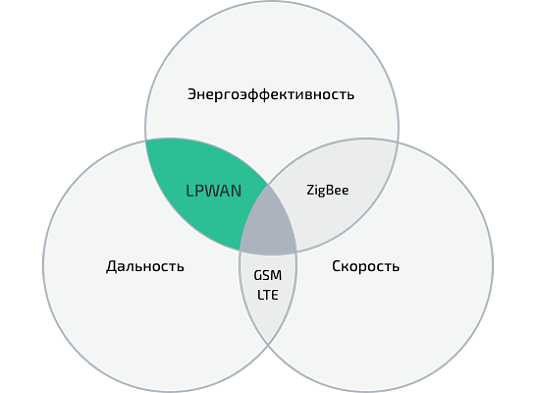
\includegraphics[width=0.7\linewidth]{pics/lpwan}
	\caption{Преимущества протоколов передачи данных}
	\label{fig:lpwan}
\end{figure}

В технологии LPWAN используется протокол XNB (Extended Narrowband). Он представляет собой переработку протокола связи на физическом уровне. XNB разработан для обмена данными устройств на больших распределенных территориях с минимальными затратами энергии.

\begin{figure}[H]
	\centering
	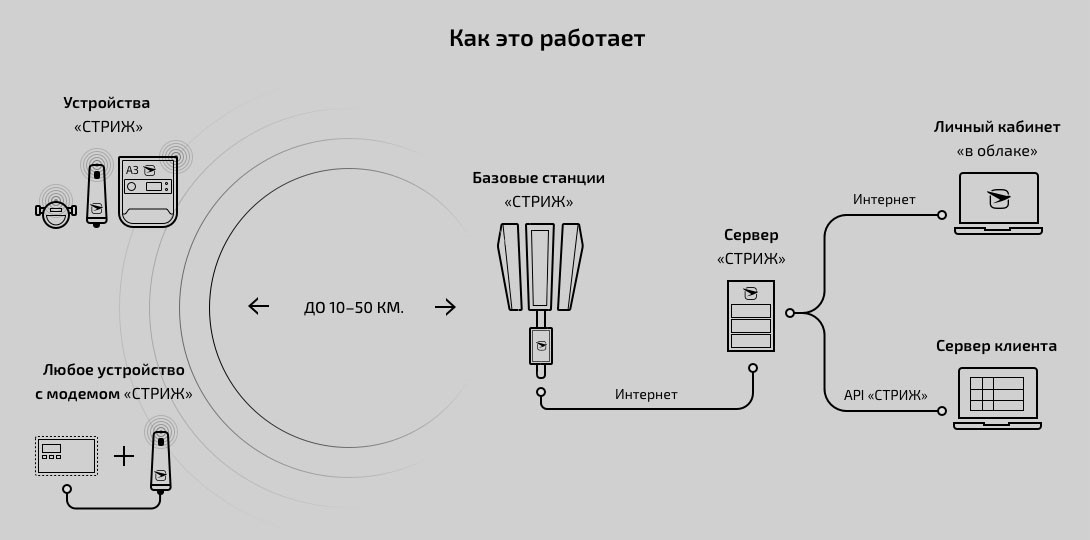
\includegraphics[width=0.7\linewidth]{pics/strij}
	\caption{Схема работы системы «СТРИЖ»}
	\label{fig:strij}
\end{figure}

Устройства и модемы «СТРИЖ» передают 8-байтные пакеты данных по беспроводному протоколу XNB на частоте 868,8 МГц (не требует лицензирования). Базовая станция принимает и обрабатывает сигналы от всех устройств «СТРИЖ» в радиусе 10—40 км.  Все станции передают данные на сервер. Сервер осуществляет обработку данных, мониторинг и управление устройств. Пользователь получает информацию в облачном личном кабинете «СТРИЖ» или по API в свое приложение.

\subsubsection{Достоинства и недостатки}

Система «СТРИЖ» обладает следующими преимуществами:

\begin{itemize}
	\item Передача данных до 50 км на открытой местности и до 10 км в городских условиях;
	\item Низкая энергозатратность, позволяет передавать данные по беспроводному каналу связи в течении нескольких лет, используя одну батарейку типа АА;
	\item Не нужно протягивать провода, позволяет устанавливать систему в уже построенные дома;
	\item Высокая проникающая способность благодаря технологии радиосвязи LPWAN;
	\item Масштабируемость, технические характеристики базовой станции позволяют подключать очень большое количество точек учета;
	\item Простота использования;
\end{itemize}

Однако у этой системы есть и свои недостатки:
\begin{itemize}
	\item Менее надежная передача данных, чем по проводному каналу; 
	\item Беспроводной канал связи подвержен индустриальным и естественным помехам;
	\item При поломке базовой станции перестаёт работать вся система до момента устранения неисправности или замены на новую станцию;
	\item Стоимость оборудования;
\end{itemize}

\subsection{АСКУЭ «Ресурс»}

АСКУЭ «Ресурс» (Автоматизированная Система Контроля и Учёта Энергоресурсов) --- это решение для удаленного автоматизированного получения показаний с приборов учёта ресурсов (воды, газа, тепла, электричества). \cite{resurce}
\subsubsection{Описание системы}

АСКУЭ «Ресурс» от ЗАО НВП Болид позволяет хранить, передавать, обрабатывать и анализировать информацию с приборов учёта ресурсов в режиме реального времени независимо от типа устройства и производителя.

Для передачи данных используются следующие стандарты интерфейсов: RS485, RS232, CAN, Meter-Bus (M-Bus), GSM/GPRS, радиоканал, Ethernet/Internet.
Данная система имеет следующие схемы подключения:
\begin{itemize}
	\item Подключение импульсных счётчиков по проводам;
	\item Подключение импульсных счётчиков по радиоканалу;
\end{itemize}

\begin{figure}[H]
	\centering
	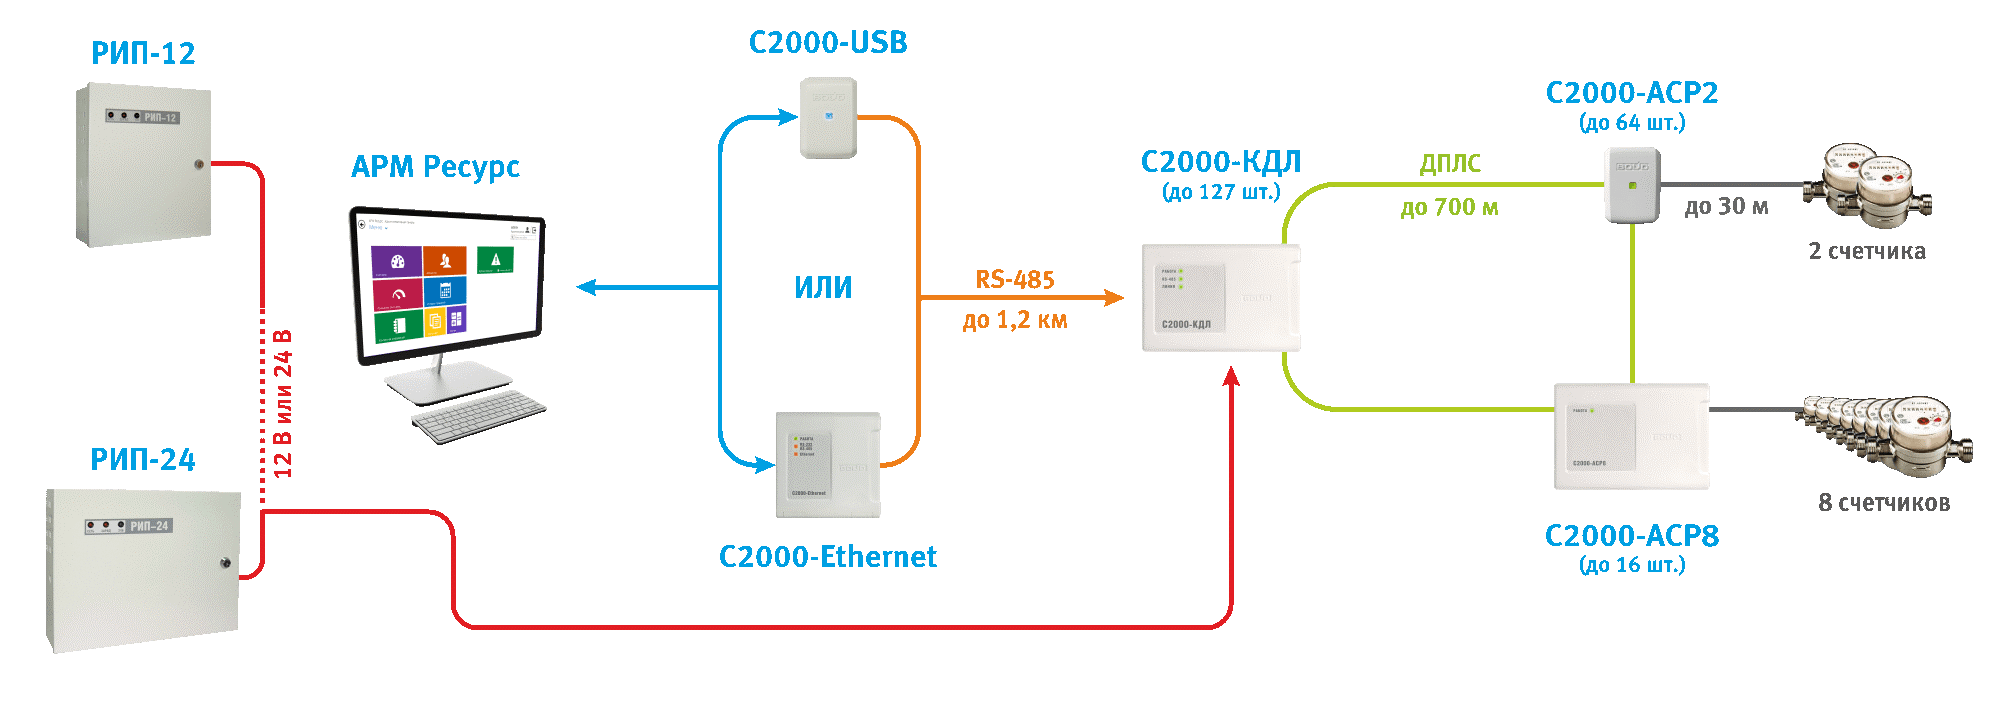
\includegraphics[width=0.7\linewidth]{pics/impuls}
	\caption{Подключение импульсных счётчиков по проводам}
	\label{fig:impuls}
\end{figure}

\begin{figure}[H]
	\centering
	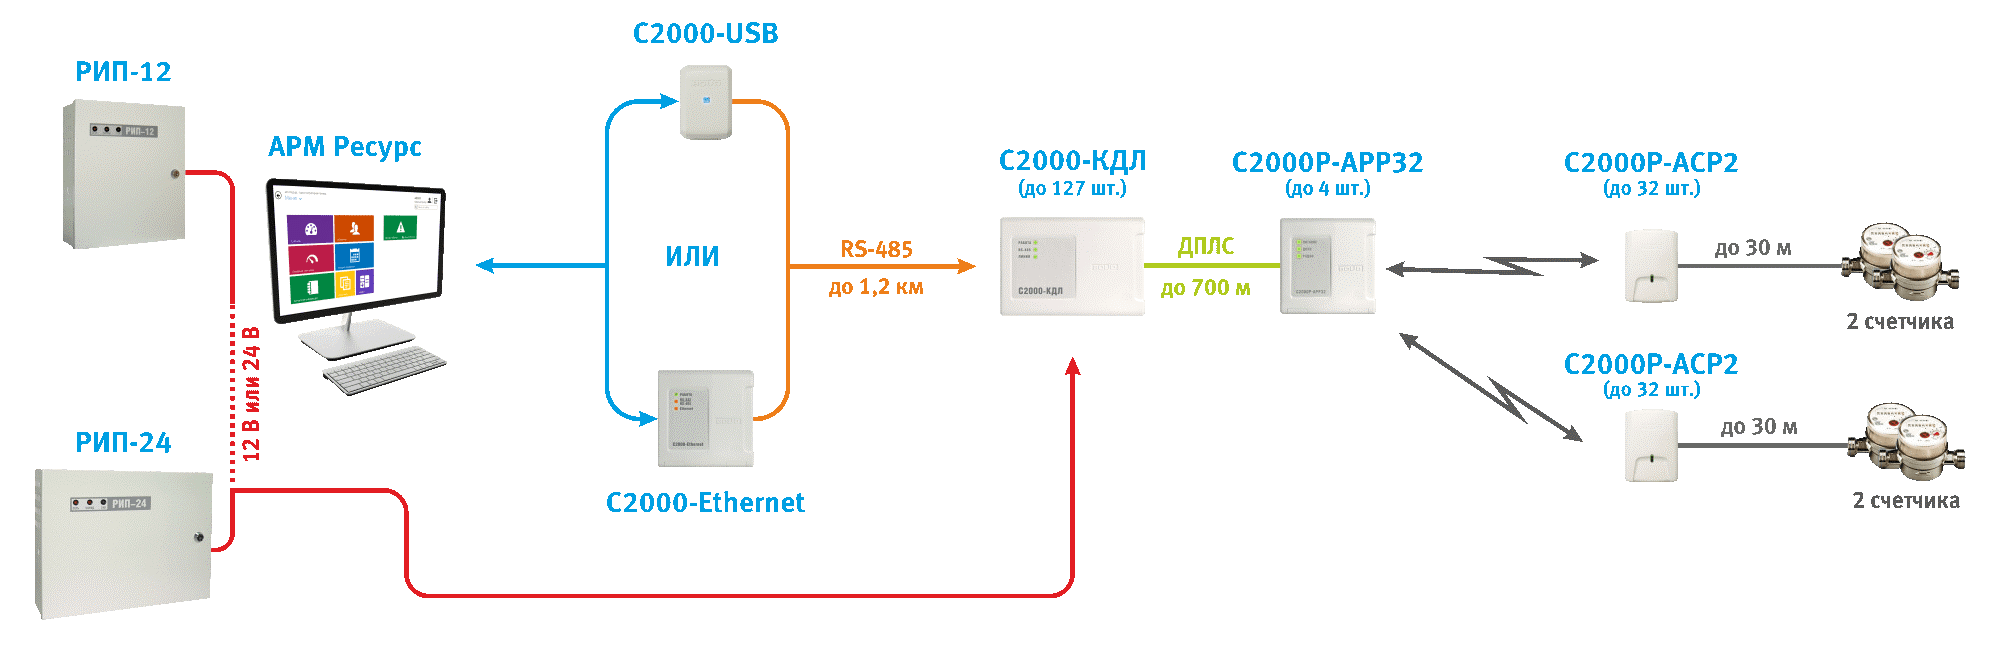
\includegraphics[width=0.7\linewidth]{pics/radio}
	\caption{Подключение импульсных счётчиков по радиоканалу}
	\label{fig:radio}
\end{figure}

\subsubsection{Достоинства и недостатки}

Достоинства:
\begin{itemize}
	\item Система имеет проводные и беспроводные решения;
	\item Наличие личного кабинета; 
	\item Возможность просматривать информацию с помощью web-интерфейса или специальной программы на компьютере;
	\item Наличие резервного питания на устройствах;
\end{itemize}
Недостатки:
\begin{itemize}
	\item Высока стоимость системы в целом из-за большого количества промежуточных устройств и преобразователей;
	\item Из-за линейного подключения устройств система имеет меньшую надежность; \item При выходе из строя одного из устройств не работает вся система;
\end{itemize}

\subsection{Сравнение и оценка}

Объекты сравниваются и оцениваются методом экспертных оценок. Выбирается ряд параметров, по которым будут оцениваться каждая система. Параметры оценивается по 10-тибальной шкале:
\begin{enumerate}
	\item Стоимость системы (1 – высокая, 10 – низкая) - сравнивается общая стоимость оборудования, технических работ и использования программного обеспечения;
	\item Надёжность системы, работоспособность системы при выходе из строя одного из устройств, а также надёжность передачи и хранения данных (1 – ненадёжная, 10 – очень надёжная);
	\item Безопасность системы (1 – система не безопасна, 10 – высокий уровень) -использование шифрования данных; защита от внешних факторов; защита от взлома; 
	\item Простота ввода системы в эксплуатацию (1 – проблемы с вводом в эксплуатацию, 10 – очень просто) - удобство ввода системы в уже построенные дома. 
	\item Простота замены комплектующих системы (1 – сложно, 10 – очень просто) - настройка нового оборудования; время замены отказавшего устройства на новое.
\end{enumerate}

\begin{table}[H]
	\caption{Сравнение и оценка системы} \label{tab:tab3}
	\centering
	\begin{tabular}{|p{1.4cm}|p{3cm}|p{1cm}|p{3cm}|p{3cm}|p{3cm}|}
		\hline 
		№ & Параметр & Вес & Система "СТРИЖ" & АСКУЭ "Ресурс" & Система "СКАУТ" \\ 
		\hline 
		1 & Стоимость & 0.3 & 2 & 6 & 8 \\ 
		\hline 
		2 & Надёжность & 0.25 & 6 & 5 & 7 \\ 
		\hline 
		3 & Безопасность & 0.1 & 8 & 5 & 5 \\ 
		\hline 
		4 & Простота ввода системы в эксплуатацию   & 0.2 & 9 & 6 & 7 \\ 
		\hline 
		5 & Простота замены комплектующих & 0.15 & 8 & 5 & 8 \\ 
		\hline 
		Сумма & & 1 & 5.9 & 5.7 & 7.05 \\ 
		\hline 
	\end{tabular} 
\end{table}
В результате система «СКАУТ» оказалась более эффективной в сравнении с другими системами.   % первая глава - в файле part1.tex
\pagebreak
% вторая часть

\section{Аппаратная часть}
\subsection{Обзор аппаратно-программного комплекса «СКАУТ»}
Обычно, жилой дом становится умным, благодаря применению в нем аппаратно-программного комплекса СКАУТ. Задача СКАУТА --- усиление безопасности, экономия ресурсов и повышение комфорта жителей. \cite{Almanah}

Функции аппаратно-программного комплекса СКАУТ можно разделить на семь, тесно связанных между собой, систем.
\begin{enumerate}
	\item Контроль доступа; 
	\item Учет ресурсов;
	\item Оповещение;
	\item Wi-Fi;
	\item Охрана технических помещений;
	\item Управление оборудованием;
	\item Видеонаблюдение.
\end{enumerate} 

Для доступа или въезда на территорию комплекса используется универсальный электронный ключ. Ключ является персональным для жителей, его копирование или подделка исключена. Все технические помещения находятся под контролем скаута. Снятие и постановка на охрану осуществляется техническим персоналом самостоятельно, с помощью мобильного телефона. Универсальный механический ключ удобен в эксплуатации и облегчает перемещение работников. 

Все потребляемые жителями ресурсы полностью учитываются и публикуются на сайте управляющей компании. Автоматизированный анализ показаний позволяет своевременно выявлять нарушении режимов отопления, неисправности приборов учета, возникающие аварии. 

Громкоговорящая система оповещения и информирования вовремя предупредит о планируемых ремонтных работах, причинах и сроках ликвидации аварийных ситуаций. Оператору управляющей компанией достаточно набрать текст сообщения и очертить на электронной карте зону оповещения. 

В чрезвычайных ситуациях диспетчер управляющей компании в ручном режиме может управлять электрооборудованием дома: шлагбаумами, электрозадвижками, системой дымоудаления, пожарными насосами.

Система видеонаблюдения, кроме охранных функций, осуществляет контроль исполнения команд диспетчера. Дает информацию о заполненности парковки на мобильные устройства. Система видеонаблюдения включена в муниципальный комплекс Безопасный город.

Используя Wi-Fi технологию, СКАУТ обеспечивает работникам управляющей компанией мобильный доступ к проектной документации, связь с диспетчером, передачу контрольной и видео информаций в аварийных случаях. 

Каждый житель цифрового района имеет доступ к данным системам СКАУТ через личный кабинет, в котором может получить видеоинформацию, организовать доступ гостей и родственников, получить информацию по коммунальным платежам. 

Умный город состоит из умных домов, а пока СКАУТ ступень к новому качеству жизни.

\subsection{Raspberry Pi 2 model B}

Благодаря своему небольшому размеру, малой стоимости, хорошей вычислительной мощности и качественной поддержке со стороны производителя в качестве главной вычислительной мощности был выбран одноплатный миникомпьютер фирмы Raspberry Pi. 

\subsubsection{Описание}

Raspberry Pi - миниатюрный одноплатный компьютер изображен на рисунке~\ref{fig:raspberry}. \cite{Raspberry} Из-за широкой функциональности и небольшой стоимости Raspberry Pi получил широкое распространение среди разработчиков и любителей электроники. Данный компьютер обладает следующими преимуществами:

\begin{itemize}
	\item Малый размер, 85,6 x 54,0 x 17 мм;
	\item Вычислительная мощность;
	\item Удобный софт и техподдержка;
	\item Малая стоимость, около 35 \$;
	\item Потребляемая мощность меньше 10 Вт;
\end{itemize}

\begin{figure}[H]
	\centering
	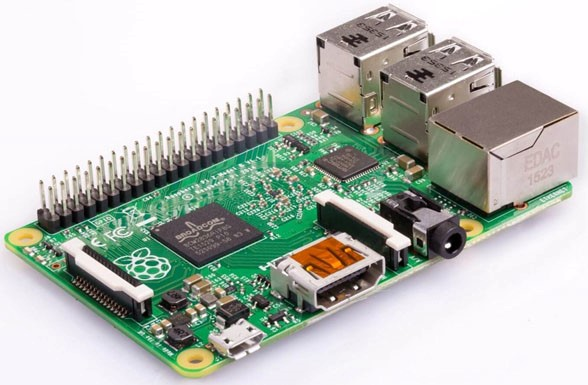
\includegraphics[width=0.7\linewidth]{pics/raspberry}
	\caption{Raspberry Pi 2 model B}
	\label{fig:raspberry} 
\end{figure}

\subsubsection{Технические характеристики}
Рассмотрим технические характеристики в таблице~\ref{tab:tab2}
\begin{table}[H]
	\caption{Технические характеристики Raspberry Pi 2 model B} \label{tab:tab2}
	\centering
	\begin{tabular}{|p{3.5cm}|p{12cm}|}
		\hline
		\multicolumn{2}{|c|}{Технические характеристики} \\
		\hline 
		Система на кристалле (SoC) & Broadcom BCM2836 (CPU + GPU) \\ 
		\hline 
		Процессор & 32-битный четырехъядерный ARMv7-A Cortex-A7 с тактовой частотой 900 МГц, 16 КБ cache L1 и 256 КБ cache L2 \\ 
		Графический процессор & Двухъядерный процессор (GPU) VideoCore IV® с тактовой частотой 250 МГц поддерживает стандарты OpenGL ES 2.0, OpenVG, MPEG-2, VC-1 и способен кодировать, декодировать и выводить Full HD-видео (1080p, 30 FPS, H.264 High-Profil) \\ 
		\hline 
		ОЗУ & 1 ГБ SDRAM LPDDR2 900 МГц EDB8132B4PB-8D-F (совместно с GPU) \\ 
		\hline 
		Хранилище & слот для карты памяти MicroSDHC, USB Boot Mode \\ 
		\hline 
		Ethernet & 10/100 Мбит с выходом на стандартное гнездо 8P8C (RJ45) (контроллер LAN9514-JZX — USB 2.0 Hub и 10/100 Ethernet) \\ 
		\hline 
		Видео вход & 1 x CSI-2 для подключения камеры по интерфейсу MIPI \\ 
		\hline 
		Видео выход & 1 x HDMI 1.3a (CEC) 1 x DSI (Display Serial Interface) для подключения штатного дисплея; 1 x композитный видеовыход (CVBS видео, PAL и NTSC) 3.5 мм разъем \\ 
		\hline 
		Аудио вход & I$^{2}$S \\ 
		\hline 
		Аудио выход & гнездо 3.5 мм, HDMI \\ 
		\hline 
		USB-порты & 4 порта USB 2.0 через USB hub в LAN9514-JZX \\ 
		\hline 
		Периферия & 40 портов ввода-вывода общего назначения (GPIO), UART (Serial), I$^{2}$C/TWI, SPI с селектором между двумя устройствами; пины питания: 3,3 В, 5 В и земля. \\ 
		\hline 
		Питание & 5 В, 2 А через порт micro-USB или GPIO \\ 
		\hline 
		Энергопотребление & 220 мА (1.1 Вт) в среднем (режиме ожидания), 820 мА (4.1 Вт) максимум, в условиях стресса (монитор, клавиатура и мышь подключены) \\ 
		\hline 
		Размеры & 85.6 мм x 56.5 мм x 17 мм \\ 
		\hline 
		Вес & 45 г \\ 
		\hline 
		ОС & Ubuntu, Debian, Fedora, Arch Linux, Gentoo, RISC OS, Android, Firefox OS, NetBSD, FreeBSD, Slackware, Tiny Core Linux, Windows 10 IOT \\ 
		\hline  
	\end{tabular}	
\end{table}

\subsection{Контроллер приборов учета}

Для подключения счётчиков был выбран контроллер приборов учета. Данный КПУ позволяет подключать до 12 счётчиков, опрашивать и хранить данные в течении длительного времени(Рисунок~\ref{fig:kpu}). Предусмотрено резервное питание при падении основного.

\subsubsection{Назначение}

Контроллер приборов учета КПУ входит в комплект инженерного оборудования жилого дома.
КПУ предназначен для подсчета количества импульсов, поступающих от подключенных водосчетчиков, электросчетчиков и теплосчетчиков, имеющих выход, выполненный по схеме «открытый коллектор» или «сухой контакт». 
Устройство предназначено для работы в следующих условиях:

\begin{itemize}
	\item Температура окружающей среды от -10$^{0}$С до 45$^{0}$С;
	\item Относительная влажность воздуха от 50\% до 80\% при 25$^{0}$С;
\end{itemize}

Питание устройства осуществляется постоянным током напряжением 9-15 В. В случае пропадания основного питания счетчик многоканальный КПУ переходит на питание от встроенного литиевого элемента напряжением 3 вольта (минимальный время работы от встроенного литиевого элемента --- 5000 часов).
Функции КПУ:

\begin{itemize}
	\item Подсчет количества импульсов, поступивших от приборов учета;
	\item Хранение значения измеряемого параметра, полученного от приборов учета, в энергонезависимой памяти;
	\item Обмен информацией с ПК по интерфейсу RS-485;
\end{itemize}
Основные технические данные представлены в таблице~\ref{tab:tab1}.
\begin{figure}
	\centering
	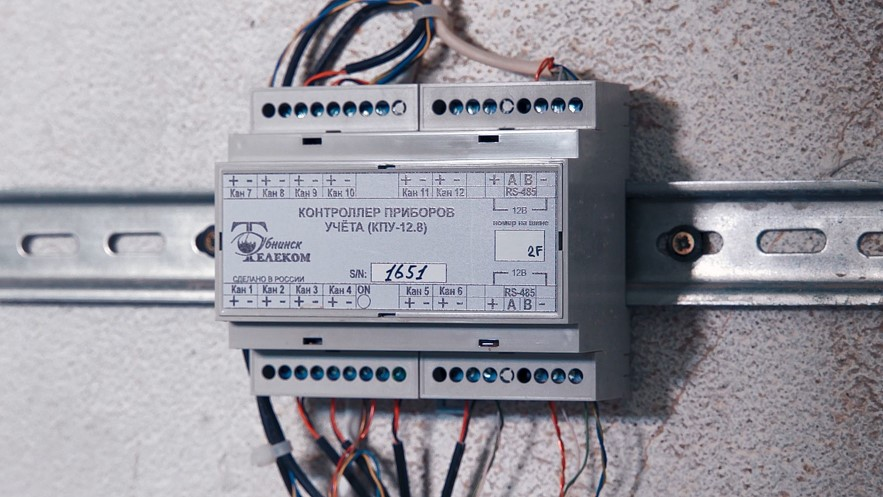
\includegraphics[width=0.7\linewidth]{pics/kpu}
	\caption{Контроллер приборов учета}
	\label{fig:kpu}
\end{figure}

\begin{table}[H]
	\caption{Технические данные КПУ} \label{tab:tab1}
	\centering
	\begin{tabular}{|p{10cm}|p{5cm}|}
		\hline 
		Максимальное количество подключаемых приборов учета & 12 \\ 
		\hline 
		Максимальное количество КПУ на шине RS485 & 128 \\ 
		\hline 
		Максимальная длина линии связи между КПУ и прибором учета, м, не более & 50 \\ 
		\hline 
		Максимальная длина линии связи между КПУ и персональным компьютером, м, не более & 1200 \\ 
		\hline
		Количество проводов между КПУ и счетчиком & 2 \\
		\hline
		Количество проводов между КПУ и персональным компьютером & 4 \\
		\hline
		Минимальное время замкнутого/разомкнутого состояния контактов датчиков, мс & 20 \\
		\hline
		Максимальное время реакции КПУ на полученную команду, мс & 50 \\
		\hline
		Количество импульсов на единицу измерения & от 10 до 2500 (кратное 10) \\
		\hline
		Потребляемая мощность, Вт, не более & 0,4 \\
		\hline
		Ресурс энергонезависимой памяти, лет & 50 \\
		\hline
		Максимально возможное хранимое показание & 999999,9 \\
		\hline
		Габаритные размеры, мм, не более & 140 x 95 x 40 \\
		\hline
		Масса блоков, кг, не более & 0,15 \\
		\hline
		Интерфейс связи с персональным компьютером & RS-485 9600 бод, 1 стоп-бит, без бита контроля \\
		\hline
	\end{tabular} 
\\Источник: документация к КПУ	
\end{table}

\subsection{Датчики}

Данные счётчики получили высокое распространение и были выбраны для использования благодаря простоте установки, малой погрешности и невысокой стоимости. 

\subsubsection{Itelma}

Счетчики Itelma для горячей и холодной воды (Рисунок~\ref{fig:itelma}). 

Счетчики на воду Ителма относятся к устройствам крыльчатого вида с механическим индикатором. Они сделаны на российских предприятиях по лицензии фирмы Siemens. Приборы изготавливают из комплектующих деталей немецкого производства. Это обеспечивает надежность и долговечность. \cite{itelma}

Устройства отличаются высокой чувствительностью, они работают при небольшом расходе воды, от 10 литров в час. Работают при давлении до 1 Мпа, диапазон температур составляет от 5 до 30 градусов для холодной воды, от 5 до 90 градусов – для горячей жидкости.

Счетчик воды WFK 24 дополнительно комплектуется импульсным датчиком с последовательным и шунтирующим (короткозамкнутым) сопротивлениями, соответствующими схеме НАМУР (NAMUR) для дистанционной передачи низкочастотных импульсов с контролем обрыва линии. \cite{saures}
Цена импульса – 0,01 м$^{3}$/имп. 

Счетчики защищены от манипулирования показаниями с помощью внешнего магнитного поля. Срок службы прибора для горячей воды составляет четыре года, для холодной воды --- шесть лет.

\begin{figure}[H]
	\centering
	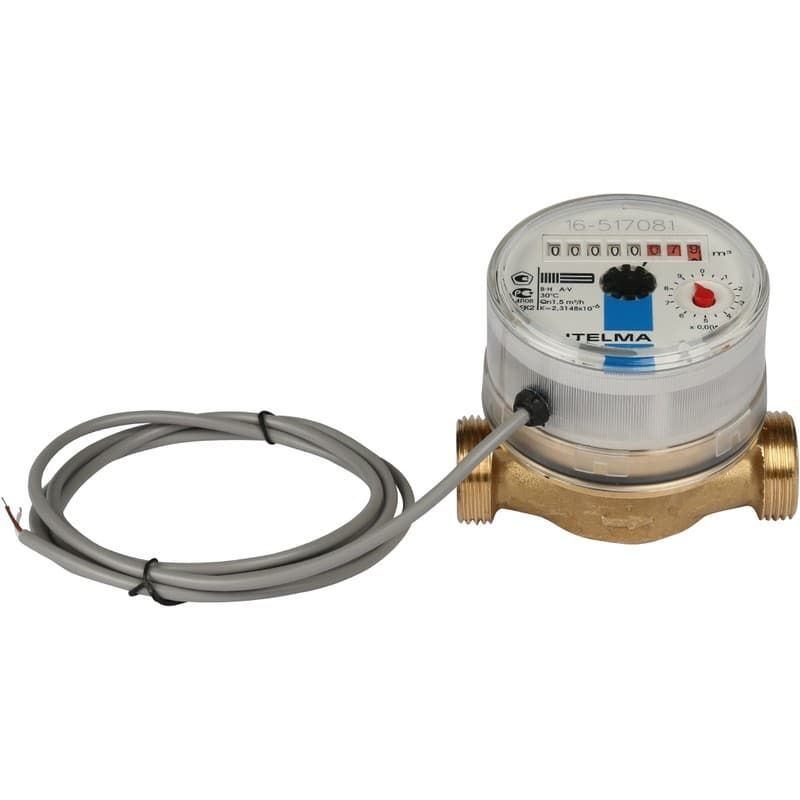
\includegraphics[width=0.5\linewidth]{pics/itelma}
	\caption{Внешний вид датчиков ITELMA}
	\label{fig:itelma}
\end{figure}

\subsubsection{SANEXT Mono}

Квартирные теплосчетчики предназначены для измерения количества потребляемой энергии в закрытых системах водяного отопления индивидуальных потребителей (поквартирный учет). Применяются при горизонтальной двухтрубной разводке системы отопления (Рисунок~\ref{fig:sanext}).

Принцип работы квартирного теплосчетчика основан на измерении расхода теплоносителя и разницы температур в подающем и обратном трубопроводах системы теплоснабжения и последующем определении количества потребленной энергии путем обработки результатов измерения вычислителем. \cite{sanext}
Преимущества механических теплосчетчиков SANEXT:

\begin{itemize}
	\item Минимальная монтажная высота, дает возможность установки теплосчетчика в небольших коллекторных шкаф или стеснённых условиях;
	\item Выносной дисплей упрощает процесс снятия показаний;
	\item Квартирные теплосчетчики с низким минимальным расход Qi от 5 л/ч подходит даже для помещений с малой площадью;
	\item Низкая потеря давления;
	\item Удобная навигация по меню счетчика;
	\item В архиве данных счётчика сохраняются ежемесячные показания счётчика в течение всего срока эксплуатации;
	\item Монтажные элементы выполнены из латуни, что обеспечивает длительный срок службы всех элементов приборов;
	\item Использование квартирных теплосчетчиков позволяет существенно экономить расход тепловой энергии;
	\item Межпроверочный интервал 6 лет;
\end{itemize}

Теплосчетчики включают в себя преобразователь расхода, вычислитель и пару платиновых термопреобразователей сопротивления.
Принцип работы теплосчетчиков состоит в измерении объема и температуры теплоносителя в подающем и обратном трубопроводах и последующем определении тепловой энергии, путем обработки результатов измерений вычислителем.

\begin{figure}[H]
	\centering
	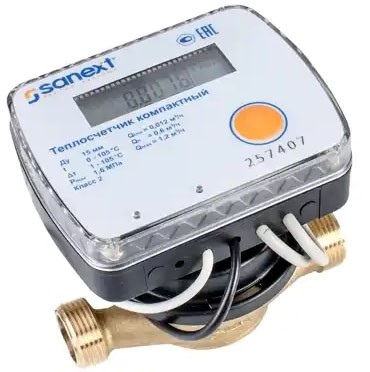
\includegraphics[width=0.4\linewidth]{pics/SANEXT}
	\caption{Внешний вид датчика SANEXT Mono}
	\label{fig:sanext}
\end{figure}

\subsubsection{Меркурий 201.5}

Счетчики ватт-часов активной энергии переменного тока электронные Меркурий 201, непосредственного включения, однофазные, однотарифные, с импульсным выходом, предназначены для измерения и учета электрической активной энергии в двухпроводных сетях переменного тока напряжением 230 В, частотой (50+-1) Гц. (Рисунок~\ref{fig:mercuriy})

Принцип действия счетчиков ватт-часов активной энергии переменного тока электронных «Меркурий 201» основан на учете информации, получаемой с импульсного выхода измерительной микросхемы. В качестве датчиков тока в счетчиках используется шунт, включенный последовательно в цепь тока. В качестве датчиков напряжения используются резистивные делители, включенные в параллельную цепь напряжения. \cite{incotexcom}

В качестве счетного механизма счетчики имеют электромеханические устройства отсчетные (УО) или жидкокристаллические индикаторы (ЖКИ) согласно таблице 1.

Счетчики с УО обеспечивают отображение информации в виде шестиразрядных чисел, пять старших разрядов дают показания в кВт-ч, шестой разряд, отделенный запятой, индицирует значение электроэнергии в десятых и сотых долях кВт-ч.

Счетчики с ЖКИ обеспечивают отображение энергопотребления нарастающим итогом в виде восьмиразрядных чисел, шесть старших разрядов дают показания в кВт-ч, два младших -указывают десятые и сотые доли кВт ч. Имеют световую индикацию мощности потребления. Период мерцания светового индикатора пропорционален уровню энергопотребления. В качестве испытательного выходного устройства счетчики имеют электрический и (или) оптический импульсный выход. Могут применяться автономно или в автоматизированных системах по сбору и учету информации о потребленной электроэнергии.  

\begin{figure}[H]
	\centering
	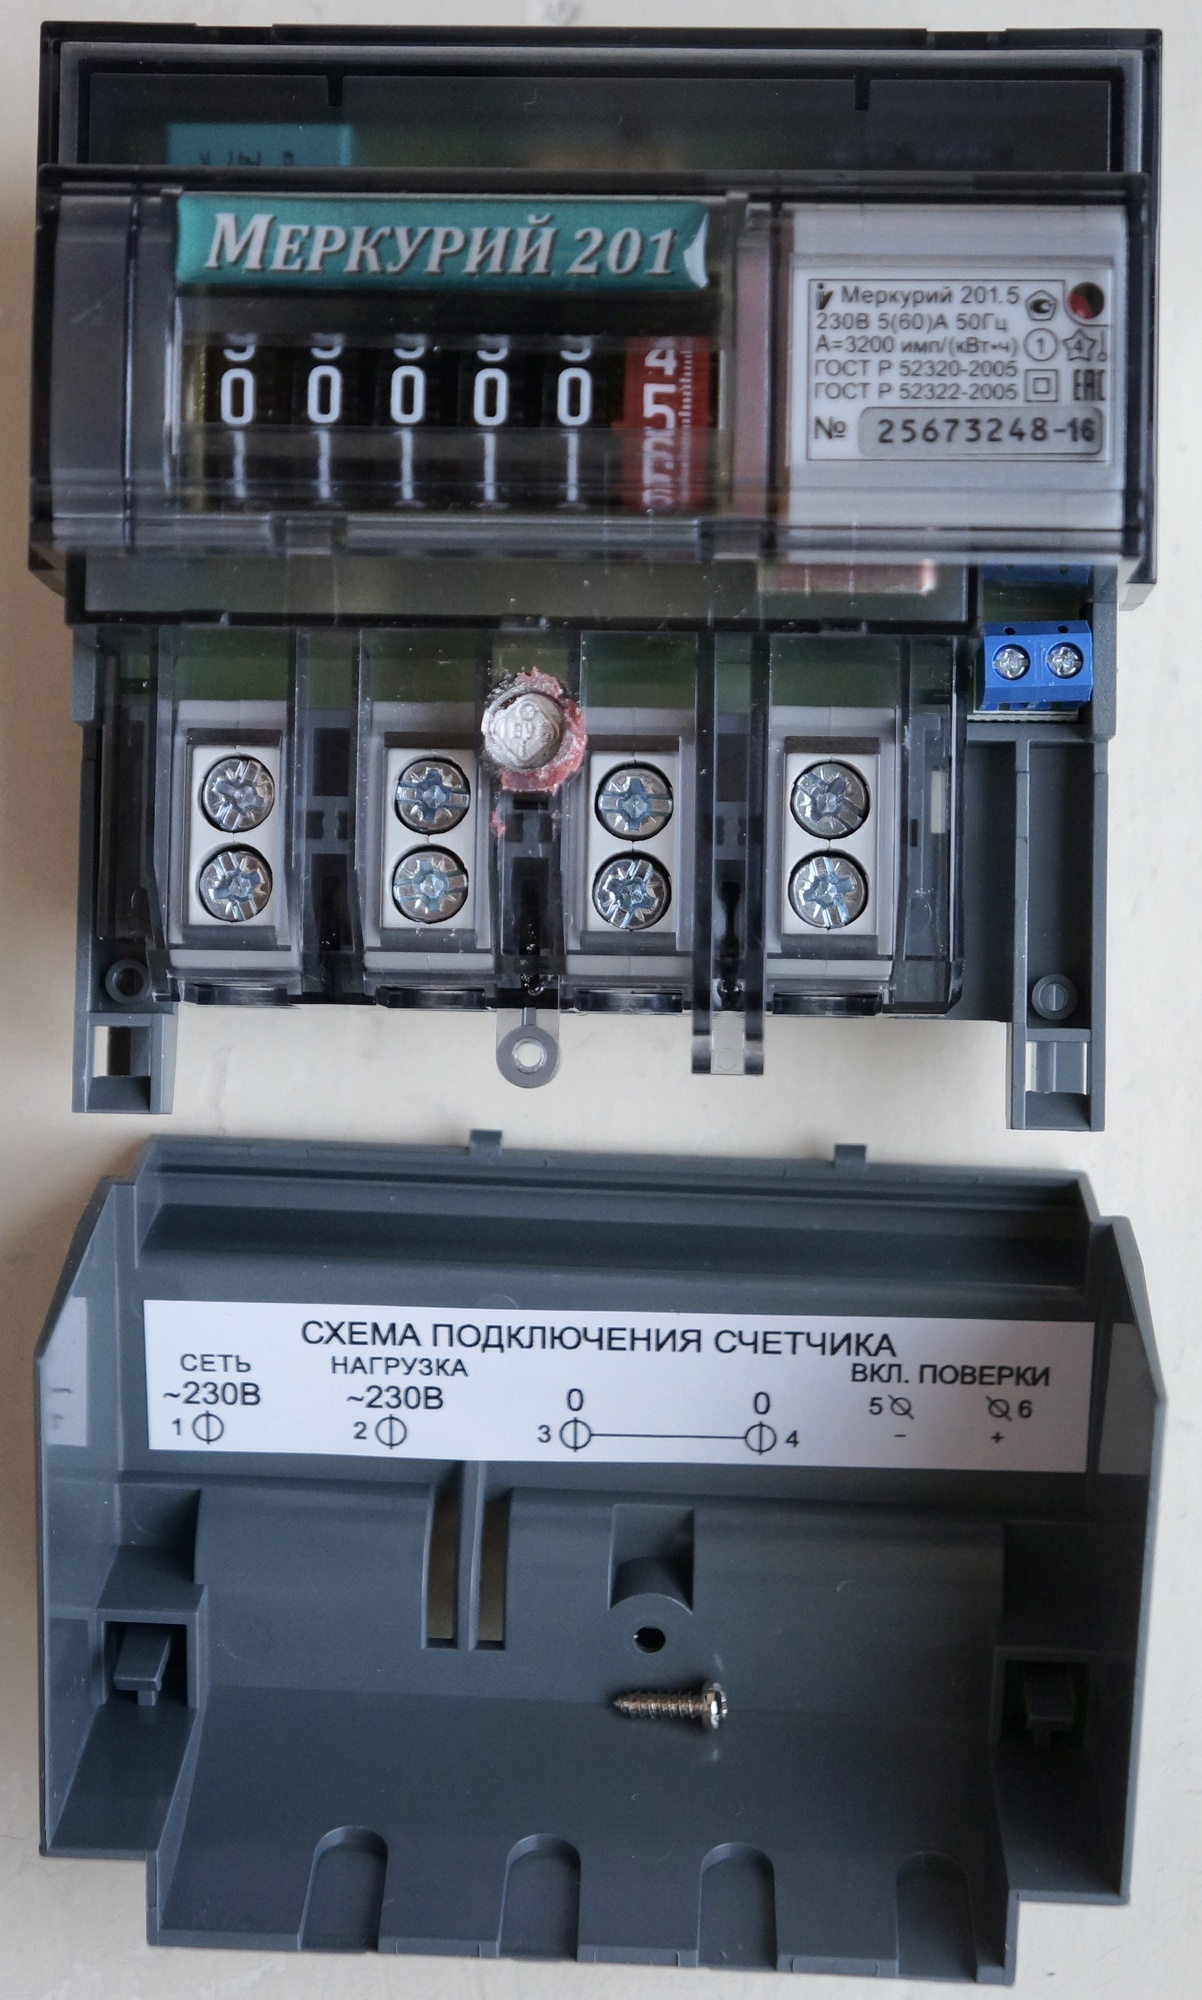
\includegraphics[width=0.5\linewidth]{pics/mercuriy}
	\caption{Меркурий 201.5}
	\label{fig:mercuriy}
\end{figure} % вторая глава - в файле part2.tex
\pagebreak

% третья часть

\section{Разработка системы квартирного учета потребления ресурсов}
Система учета ресурсов предназначена для считывания, мониторинга и работы с данными домовых счетчиков учета ресурсов. Данные со счетчиков попадают на сервер баз данных, в программе диспетчера и администратора данные отображаются, считаются, формируются отчеты. \cite{NK}

Проблемы:  
\begin{itemize}
	\item Некорректные начисления по оплате; 
	\item Неверная работа квартирных приборов учета (неисправности, воровство); 
	\item поставка ресурсов ненадлежащего качества (недогрев, перегрев, некачественная электроэнергия);
	\item Некорректная работа регулирующего теплового оборудования; 
	\item Отсутствие технической возможности проводного соединения с квартирными приборами учета.
\end{itemize}

Решение: 
\begin{enumerate}
	\item Создание единой облачной базы данных; 
	\item Конвертирование архивов ПУ различных производителей;
	\item Автоматизированный анализ данных.
\end{enumerate}

Система учета ресурсов состоит из:
\begin{itemize}
	\item Сервера баз данных;
	\item Контроллеры приборов учёта;
	\item Преобразователей интерфейса;
	\item Домовой сервер (Raspberry Pi);
	\item Службы сбора данных;
	\item Управляющей программы(администратора и диспетчера).
\end{itemize}
Администратор системы должен контролировать состояния на панеле мониторинга, добавлять новые счетчики, составлять отчеты, проводить аналитику. 

\subsection{Формирование единой базы данных}

\begin{enumerate}
	\item Опросом показаний занимается программа, запущенная на домовом сервере (Raspberry Pi).  Она должна извлекать данные о требуемых к опросу счетчиках из текстового файла (приложение 1.1), производить опрос и сохранять показания в отдельный текстовый файл (приложение 1.2). Опрос показаний должен производится 1 раз  в час (например в 05 минут каждого часа).
	\item Служба сбора данных производит непосредственный опрос всех Raspberry Pi. Эта программа устанавливается на сервер баз данных и производит выгрузку файлов data.txt  с домовых серверов в единую базу данных (FireBird, PostgreSQL) (приложение 2). После занесения данных в основную базу необходимо очистить файл data.txt.  Если в основной базе изменилась информация о счетчиках (порт, адрес КПУ или номер клеммы) данная программа должна загрузить новый файл counter.txt.
	\item Раз в сутки необходимо синхронизировать время домового сервера и сервера БД (это может быть отдельная программа или одна из функций программы из п.2).	
\end{enumerate}

\textbf{Квартирный учет ресурсов}

В квартирном учете применена проводная система снятия показаний. Для снятия показаний приборов учета с импульсным выходом применяется универсальный счетчик СКАУТ-КПУ, поддерживающий 12 импульсных входов. Приборы с протоколами передачи данных RS485, ModBUS и другими подключаются к плате сопряжения протоколов СКАУТ.

\textbf{Домовой учет ресурсов}

Домовые приборы учета с импульсным выходом применяются в комплекте со счетчиком импульсов СКАУТ-КПУ. При наличии у приборов внутреннего архива, опрос приборов и промежуточное хранение файлов архива осуществляется микрокомпьютером СКАУТ-Базовый

\subsection{монтаж: установка оборудования}

\begin{enumerate}
	\item Установить комплекс СКАУТ базовый в защитный шкаф
	\item Установить контроллер приборов учета
	\item Установить "умные" счетчики, с системой телеметрии на каждый вид ресурсов (газ, электроэнергия, вода, тепло)
	\item Проложить коммутационные кабели и подключить оборудование к сети связи
	\item Установить программное обеспечение на компьютер сотрудника УК
	\item Создать базы данных по счетчикам и адресам; провести пуско-наладочные работы
	\item Провести инструктаж сотрудников УК по использованию системы учета ресурсов
\end{enumerate}  % третья глава - в файле part3.tex
\pagebreak

% четвертая часть

\section{Разработка программного обеспечения системы учета ресурсов}
\subsection{Назначение}
Основная задача разрабатываемой программы упростить учет и администрирование контроллеров и приборов учета, а также своевременный анализ данных, для выявления неисправных оборудований. Составления отчетов для ЖКХ.

Полный функционал программного обеспечения:
\begin{itemize}
	\item Добавление, редактирование и просмотр оборудований СКАУТ;
	\item Просмотр замененных КПУ и ПУ;
	\item Добавление, редактирование, замена и просмотр контроллеров приборов учета; 
	\item Просмотр истории редактирования КПУ; 
	\item Добавление, редактирование, замена и просмотр приборов учета; 
	\item Добавление стартовых значений; 
	\item Просмотр часовых показаний за выбранный период; 
	\item Просмотр истории редактирования ПУ;
	\item Просмотр приборов учета имеющих короткое замыкание или обрыв линии;
	\item Автоматический анализ данных на выявление проблемных счетчиков;
\end{itemize}

Программа включает 6 основных разделов.
\begin{enumerate}
	\item Раздел - Главное меню
	\item Раздел - СКАУТ
	\item Раздел - Контроллеры Приборов Учета
	\item Раздел - Приборы Учета
	\item Раздел - Контроль линии
	\item Раздел - Проблемные счетчики
\end{enumerate}

\subsection{Описание разделов программы}
\subsubsection{Главное меню}
Раздел «Главное меню» открывается при запуске программы. Отображаются две таблицы со списком замененных КПУ и ПУ. Из вкладки «Оборудование» можно перейти в разделы «СКАУТ», «КПУ», «ПУ». Из вкладки «Анализ данных» можно перейти в раздел «Контроль линии» и «Проблемные счетчики».

\subsubsection{СКАУТ}
Раздел «СКАУТ» открывается из главного меню, вкладки «Оборудование». Отображается список подъездов, где установлен СКАУТ. 
\begin{enumerate}
	\item Кнопка «Обновить» применяет выбранные фильтры к таблице;
	\item Кнопка «Добавить» открывает форму для заполнения данных для нового СКАУТА;
	\item Двойное нажатие на строчку из таблицы. Открывается полная информация по выбранному СКАУТу. При нажатии кнопки «КПУ» откроется список КПУ подключенных к данному СКАУТу;
\end{enumerate}

\subsubsection{КПУ или Контроллеры Приборов Учета}
Раздел «КПУ» открывается из главного меню, вкладки «Оборудование» и через нажатие на кнопку «КПУ» в форме «Информация о СКАУТ». Отображается список установленных КПУ.
\begin{enumerate}
	\item Кнопка «Обновить» применяет выбранные фильтры к таблице;
	\item Кнопка «Добавить» открывает форму для заполнения данных для нового КПУ;
	\item Двойное нажатие на строчку из таблицы. Открывается информация по выбранному КПУ. Можно переключиться на вкладку «История редактирования», где отображается таблица с информацией о редактировании данных выбранного КПУ. При нажатии кнопки «ПУ» откроется список ПУ подключенных к данному КПУ;
	\item Кнопка «Заменить». Используется, когда заменили установленный КПУ на другой. Если при замене на новом КПУ указали такие же импульсы, какие были на старом, и не требуется менять показания на всех ПУ подключенных к данному КПУ, тогда убираем галочку «с заменой стартовых значений». Если указали нулевые импульсы на все клеммы, то требуется заменить стартовые значения. Выбираем время и нажимаем обновить. Отобразятся показания, номера квартир и тип ПУ на выбранную дату для старого КПУ. Если на указанное время КПУ был неисправен и показания в БД не записывались, тогда отобразятся последние сохранившиеся данные;
\end{enumerate}	

\subsubsection{ПУ или Приборы Учета}
Раздел «ПУ» открывается из главного меню, вкладки «Оборудование» и через нажатие на кнопку «ПУ» в форме «Информация о КПУ». Отображается список установленных ПУ. 
\begin{enumerate}
	\item Кнопка «Обновить» применяет выбранные фильтры к таблице;
	\item Кнопка «Добавить» открывает форму для заполнения данных для нового ПУ. Если квартиры еще нету в БД, то откроется форма для добавления новой квартиры;
	\item Двойное нажатие на строчку из таблицы. Открывается информация по выбранному ПУ. Если нужно добавить дату установки и демонтажа, то нажать на кнопку «Дата установки отсутствует» и «Дата демонтажа отсутствует»;
	\item Вкладка «Информация». При нажатии кнопки «ПУ» откроется список ПУ подключенных к данному КПУ;
	\item Кнопка «Заменить». Используется, когда заменили установленный ПУ на другой. Выбираем время, когда сняли показания с нового ПУ и нажимаем «Установить импульсы на выбранную дату», чтобы автоматически заполнились имеющиеся импульсы на подключенной клемме. Если серийный номер нового ПУ уже имеется в БД, то покажется предупреждение об этом. Если ПУ нигде не установлен, то предложит продолжить замену;
	\item Вкладка «Стартовые значения». Отображается таблица с информацией о добавленных стартовых значения для выбранного ПУ. Можно добавить новое стартовое значение;
	\item Вкладка «Показания». Отображается таблица с часовыми показаниями выбранного ПУ. По умолчанию за последние сутки. Можно изменить временной промежуток и нажать кнопку «Показать»;
	\item Вкладка «История редактирования». Отображается таблица с информацией о редактировании данных выбранного ПУ;
\end{enumerate}
	
\subsubsection{Контроль линии}
Раздел «Контроль линии» открывается из главного меню, вкладки «Анализ данных». Отображается список проблемных ПУ за последние сутки. Если столбец line\_state = 1, тогда произошел обрыв линии или короткое замыкание на линии от ПУ до КПУ. Столбец empty = 1 означает что данные не обновились. 
\subsubsection{Проблемные счетчики}
Раздел «Проблемные счетчики» открывается из главного меню, вкладки «Анализ данных». Отображается список проблемных ПУ за последние трое суток. Пользователь может выбрать свой промежуток времени. При двойном нажатие на строчку из списка откроется информационное окно с удобными, для анализа показаний, графиками потребления всех видов ресурсов выбранной квартиры. 
\subsection{Разработка программы}
\subsubsection{PyQT5}
PyQt5 --- это набор Python-связей для фреймворка Qt5 от Digia. Набор PyQt5 доступен для Python 2.x и 3.x. В моей программе используется Python 3. Библиотека Qt – это одна из самых мощных GUI-библиотек. PyQt5 разработан компанией Riberbank Computing.\cite{Python}

PyQt5 реализован как комплект Python-модулей. Он включает в себя около 620 классов и 6000 функций и методов, включая:
\begin{enumerate}
	\item Существующий набор виджетов графического интерфейса;
	\item Стили виджетов;
	\item Доступ к базам данных с помощью SQL (ODBC, MySQL, PostgreSQL, Oracle);
	\item QScintilla, основанный на Scintilla виджет текстового редактора;
	\item Поддержку интернационализации (i18n);
	\item Парсер XML;
	\item Поддержку SVG;
	\item Интеграцию с WebKit, движком рендеринга HTML;
	\item Поддержку воспроизведения видео и аудио;
\end{enumerate}
Это мульти-платформенный инструментарий, который запускается на большинстве операционных систем, среди которых Unix, Windows и MacOS. PyQt5 реализован под двумя лицензиями. Разработчики могут выбрать между GPL и коммерческой лицензией.

PyQt также включает в себя Qt Designer (Qt Creator) — дизайнер графического интерфейса пользователя. Программа pyuic генерирует Python код из файлов, созданных в Qt Designer. Это делает PyQt очень полезным инструментом для быстрого прототипирования. Кроме того, можно добавлять новые графические элементы управления, написанные на Python, в Qt Designer.\cite{PyQt5}
\subsubsection{fdb}
FDB - это пакет библиотеки Python, реализующий поддержку Python Database API 2.0 для реляционной базы данных с открытым исходным кодом Firebird. В дополнение к минимальному набору функций стандартного API Python DB, FDB также предоставляет полный нативный (в старом стиле) клиентский API ядра базы данных и ряд дополнительных расширений и улучшений для удобного использования Firebird.\cite{fdb}

FDB разрабатывается в рамках с проектом Firebird, и используется внутренне как ключевой компонент для Firebird QA.\cite{firebird}

Доступ к базе данных осуществляется через объекты подключения. FDB предоставляет два конструктора для них:
\begin{enumerate}
	\item create\_database () --- создание базы данных данных;
	\item connect () --- создание подключения к базе данных;
\end{enumerate}
Для дальнейшего общение с базой нужно получить курсор. Пример добавления нового элемента в таблицу
\begin{MyCode}
import psycopg2
conn = psycopg2.connect(dbname='database', user='user', 
password='mypassword', host='localhost')
cur = conn.cursor()
cur.execute("insert into KPU (SER\_NUM, ADRESS) values (?,?)",
		(1784, 1))
conn.commit()
cur.close()
conn.close()
\end{MyCode}
\subsubsection{psycopg2}
PostgreSQL, пожалуй, это самая продвинутая реляционная база данных в мире Open Source Software. По своим функциональным возможностям она не уступает коммерческой БД Oracle и на голову выше собрата MySQL.\cite{psycopg}

В Python самой популярной библиотекой для работы с PostgreSQL является psycopg2. Эта библиотека написана на Си на основе libpq, соответствует стандарту DB-API 2.0. Основные методы DB-API, позволяющие полноценно работать с базой данных представлены на рис.~\ref{fig:pythondb-api}

\begin{figure}[H]
	\centering
	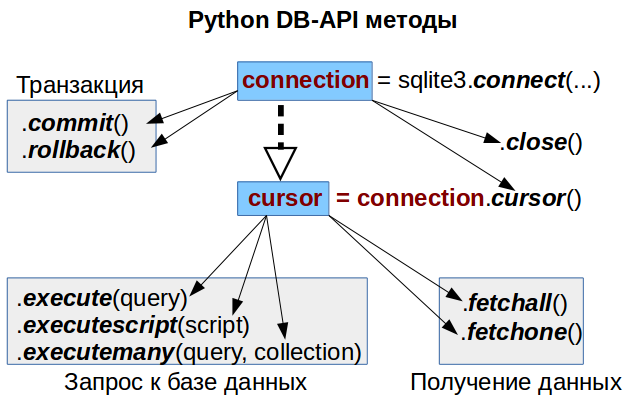
\includegraphics[width=0.7\linewidth]{pics/pythonDB-API}
	\caption{Python DB-API Методы}
	\label{fig:pythondb-api}
\end{figure}
 

 % четвертая глава - в файле part4.tex
\pagebreak

% пятая часть

\section{Реализация программного обеспечения по контролю приборов учета}

Система учета ресурсов предназначена для считывания, мониторинга и работы с данными домовых счетчиков учета ресурсов. Данные со счетчиков попадают на сервер баз данных, в программе диспетчера и администратора данные отображаются, считаются, формируются отчеты.

Полный функционал программного обеспечения:
\begin{itemize}
\item управление адресами и объектами установки ПУ;
\item управление приборами учета;
\item управление абонентами; 
\item просмотр показаний ПУ за выбранный интервал времени; 
\item расчет потребления энергоресурсов по основным показаниям ПУ за указанный интервал времени; 
\item просмотр детальной информации по потреблению энергоресурсов конкретного ПУ с выводом графика потребления; 
\item предоставление сведений об аварийных и нештатных ситуациях ПУ; 
\item экспорт полученных данных в другие форматы, вывод на печать;
\item поиск.
\end{itemize}

Программа включает 9 основных разделов.
\begin{enumerate}
	\item Раздел - Показания приборов
	\item Раздел - Состояние приборов учета
	\item Раздел - Адреса
	\item Раздел - Абоненты
	\item Раздел - Приборы учета
	\item Раздел - Лицевые счета
	\item Раздел - Отчеты
	\item Раздел - Поиск
	\item Раздел - Оповещение об ошибках и нештатных ситуациях
\end{enumerate}

Система должна быть защищенной и поэтому используются локальные данные. Сервер, база данных на постгрессе и программы на компьютерах администраторов для управления. 

\textbf{Цели:} Сбор данных и мониторинг потребления ресурсов.
 
\textbf{Задачи:}  Создать защищенную и удобную систему  для сбора данных потребляемых населением.

Программа для администратора: мониторинг, добавление/ изменение/ удаление счетчиков, составление отчетов. 

Функции программы диспетчера:

Ведение списка пользователей и управление их полномочиями;
Конфигурация для сохранения, изменения и отображать данных о подключении счетчика к конкретной КПУ (порт, адрес, клемма, коэффициент --- цены импульса). 
\begin{itemize}
	\item Ведение служебных справочников (список адресов, типов приборов и т.д.);
	\item Ввод и редактирование данных о подключенных контроллерах;
	\begin{enumerate}
		\item Создание прикрепленных индивидуальных приборов учёта с указанием:
		\begin{enumerate}
			\item номера клеммы; 
			\item цены импульса; 
			\item типа прибора;
			\item серийного номера; 
			\item единиц измерения;
			\item начального показания;
			\item номера квартиры;
			\item ФИО собственника;
		\end{enumerate}
		\item Для счётчиков требующих проверки указать дату предыдущей и следующей поверки;
		\item Групповые операции с устройствами;
	\end{enumerate}
	\item Просмотр показаний приборов учёта в табличном и графическом виде;
	\begin{enumerate}
		\item Отображение сведений о наличии или отсутствии показаний за выбранный период для выбранных устройств;
	\end{enumerate}
	\item Формирование отчетов по потреблению ресурсов --- ежемесячный отчет установленного формата для управляющей компании/ресурсоснабжающей организации;
	\item Сравнение суммарного квартирного потребления и общедомового.
	
\end{itemize}  % пятая глава - в файле part5.tex
\pagebreak

\section*{\centering ЗАКЛЮЧЕНИЕ}
\addcontentsline{toc}{section}{ЗАКЛЮЧЕНИЕ}

В России интерес к тематике Умного города растет с каждым годом, в том числе потому, что многие города подходят к пределам надежности и функциональности существующей инфраструктуры.

По результатам исследования, было рассмотрено несколько проектов Умный город. Выделены три группы проблем при разработке и реализации концепции Умного города в России. Изучены перспективы развития Умного города в Обнинске.

Проведен обзор функций аппаратно-программного комплекса СКАУТ.

Разработана система квартирного учета потребления ресурсов. 

Сформирована единая база данных. 

Проведен анализ показаний квартирных и домовых приборов учета, с помощью основных алгоритмов поиска проблемных счетчиков электроэнергии и водоснабжения. Разработан автоматизированный анализ данных.

Реализовано программное обеспечение по контролю приборов учета.

В связи с тем, что большинство современных счетчиков поддерживает протокол ModBus, появилась возможность усовершенствования системы и переноса отработанных алгоритмов анализа на web-платформу. Также планируется реализация новых задач анализа данных.

% оформление библиографии - вариант с БД
\pagebreak

\addcontentsline{toc}{section}{СПИСОК ИСПОЛЬЗОВАННОЙ ЛИТЕРАТУРЫ}
% ВАЖНО: для корректного отображения в списке литературы ссылок на англ.языке в bibtex-описание источника следует добавить поле 
% langid = {english}
\printbibliography

\pagebreak

\section*{ \centering Приложение А} 
\addcontentsline{toc}{section}{Приложение А}

\begin{center}
Листинг 1 -- Часть кода реализации класса \verb|HashMapValue|
\end{center}


\begin{MyCode}

public class HashMapValue {
	
	protected String filename; 
	protected HashMap<String, String> hashValue = 
	new HashMap<>();
	protected HashMap<String, Boolean> hashKeysFlag =
	 new HashMap<>();
	
	public void setData(String key, String value) {
		hashValue.put(key, value);
	}
	
	public String getData(String key) {
		return hashValue.get(key);
	}
    /* ... */
}
\end{MyCode}

\end{document}          

